\documentclass[a4paper]{extarticle}
\usepackage[utf8]{inputenc}
\usepackage[a4paper, margin=1in]{geometry}

\usepackage{amssymb}
\usepackage{amsmath}
\usepackage{enumitem}
\usepackage{tcolorbox}
\usepackage{fancyhdr}
\usepackage{graphicx}
\usepackage{float}

\setlength{\parindent}{0em}
\setlength{\parskip}{0.4em}

\definecolor{theoremblue}{RGB}{1, 73, 124}
\definecolor{corollaryblue}{RGB}{70, 143, 175}
\definecolor{exampleblue}{RGB}{137, 194, 217}

\newtcolorbox{tbox}{colback=theoremblue!20,colframe=theoremblue,
boxrule=0pt,arc=0pt,boxsep=2pt,left=2pt,right=2pt,leftrule=2pt}

\newtcolorbox{cbox}{colback=corollaryblue!20,colframe=corollaryblue,
boxrule=0pt,arc=0pt,boxsep=2pt,left=2pt,right=2pt,leftrule=2pt}

\newtcolorbox{ebox}{colback=exampleblue!20,colframe=exampleblue,
boxrule=0pt,arc=0pt,boxsep=2pt,left=2pt,right=2pt,leftrule=2pt}

\title{EnpRisk - Lecture Notes Week 1}
\author{Ruben Schenk, ruben.schenk@inf.ethz.ch}
\date{\today}

\pagestyle{fancy}
\fancyhf{}
\rhead{ruben.schenk@inf.ethz.ch}
\rfoot{Page \thepage}
\lhead{EnpRisk - Lecture Notes Week 1}

\begin{document}

\maketitle
\newpage

\section{Introduction}

\subsection{Entrepreneurship}

\subsubsection{Definitions}

\begin{tbox}
    \textbf{Definition:} We might define \textbf{entrepreneurship} by the following three key-ideas:

    \begin{itemize}
        \item Pursuit of opportunity without regard to resources controlled.
        \item Process of creating value through unique resource combinations that exploit opportunity.
        \item A way of thinking and acting, a lot of different professional contexts, but also a way of approaching personal issues, family, life, community involvement, etc.
    \end{itemize}
\end{tbox}

\textbf{Qualities} of an entrepreneur may include optimism, self-confidence, social networking, low risk aversion, charism, and most importantly the \textit{drive to improve} and to \textit{change the world.}

\subsubsection{Success}

There are three steps to \textit{succeeding in life,} however you define success yourself:

\begin{enumerate}
    \item Know what you want in life. Know your end goals.
    \item Write down your intermediate goals and a plan to reach these goals.
    \item Review and revise your plan monthly, keeping track of all setbacks and progress.
\end{enumerate}

\begin{cbox}
    \textit{"All success begins with something definite that you fully intend to do. Success is a function of definiteness of purpose."} - Napoleon Hill
\end{cbox}

\subsubsection{Motivation}

\textbf{Motivation} is what explains why people or animals initiate, continue or terminate a certain behavior at a particular time. In general, motivation is the reason or reasons for acting or behaving in a particular way and the desire or willingness to do something.

\subsection{Risks}

\subsubsection{Definition}

A \textbf{risk} is a potential event with negative consequences that has not happened yet. However, a risk could also be defined as the event with unforeseen positive consequences!

A risk is therefore the \textit{possibility of loss,} but not the loss itself. In other words, a source of problem during a project, but not the cost of a risk.

\subsubsection{Types of Risks}

We can distinguish risks into different types:

\paragraph{Industrial Risks}

\begin{itemize}
    \item Change in technology, productivity, and prices
    \item False estimates of the rated capacity
    \item Time needed for the construction and running-in periods, political, social, and business environment
\end{itemize}

\paragraph{Operational Risks}

\begin{itemize}
    \item Lack of entrepreneurial skills
    \item Poor understanding of market dynamics
    \item Poorly available consultancy services and information systems
    \item Poor understanding of how to prepare a business plan
    \item Natural risks
\end{itemize}

\paragraph{Market Risks}

\begin{itemize}
    \item Unforeseeable inflation and exchange rates change
    \item Customer behaviors to buy foreign goods
    \item Inadequate infrastructure
    \item Shrinking market because of foreign competitors
    \item Defaulting or insolvency, credit risks
\end{itemize}

\paragraph{Other Risks}

We furthermore can consider risks from the following categories:

\begin{itemize}
    \item Cultural risks
    \item Natural risks
    \item Economic and political risks
\end{itemize}

\subsubsection{Formal Representation}

Risk is commonly measured as a pair of the probability of occurrence of an event, and the outcomes or consequences associated with the event's outcome. This pairing can be represented by the following equation:

\[
    \text{Risk} \equiv [(p_1,c_1), \, (p_2,c_2),..., \, (p_n,c_n)],
\]

where:

\begin{itemize}
    \item \(p_i\) = occurrence probability of an outcome or event \(i\)
    \item \(c_i\) = occurrence consequences or outcomes of the event \(i\)
\end{itemize}

\subsubsection{Other Technical Terms}

Other technical terms are needed for presenting risk-based technology methods and analytical tools include:

\paragraph{Hazard} A \textbf{hazard} is an act or phenomenon posing potential harm to some person(s) or thing(s), i.e. a source of harm, and its potential consequences. Hazards need to be identified and considered in a projects' lifecycle analyses since they could pose thread and could lead to project failures.

\paragraph{Uncertainty} We introduce the term \textbf{uncertainty} with the following table:

\begin{figure}[H]
    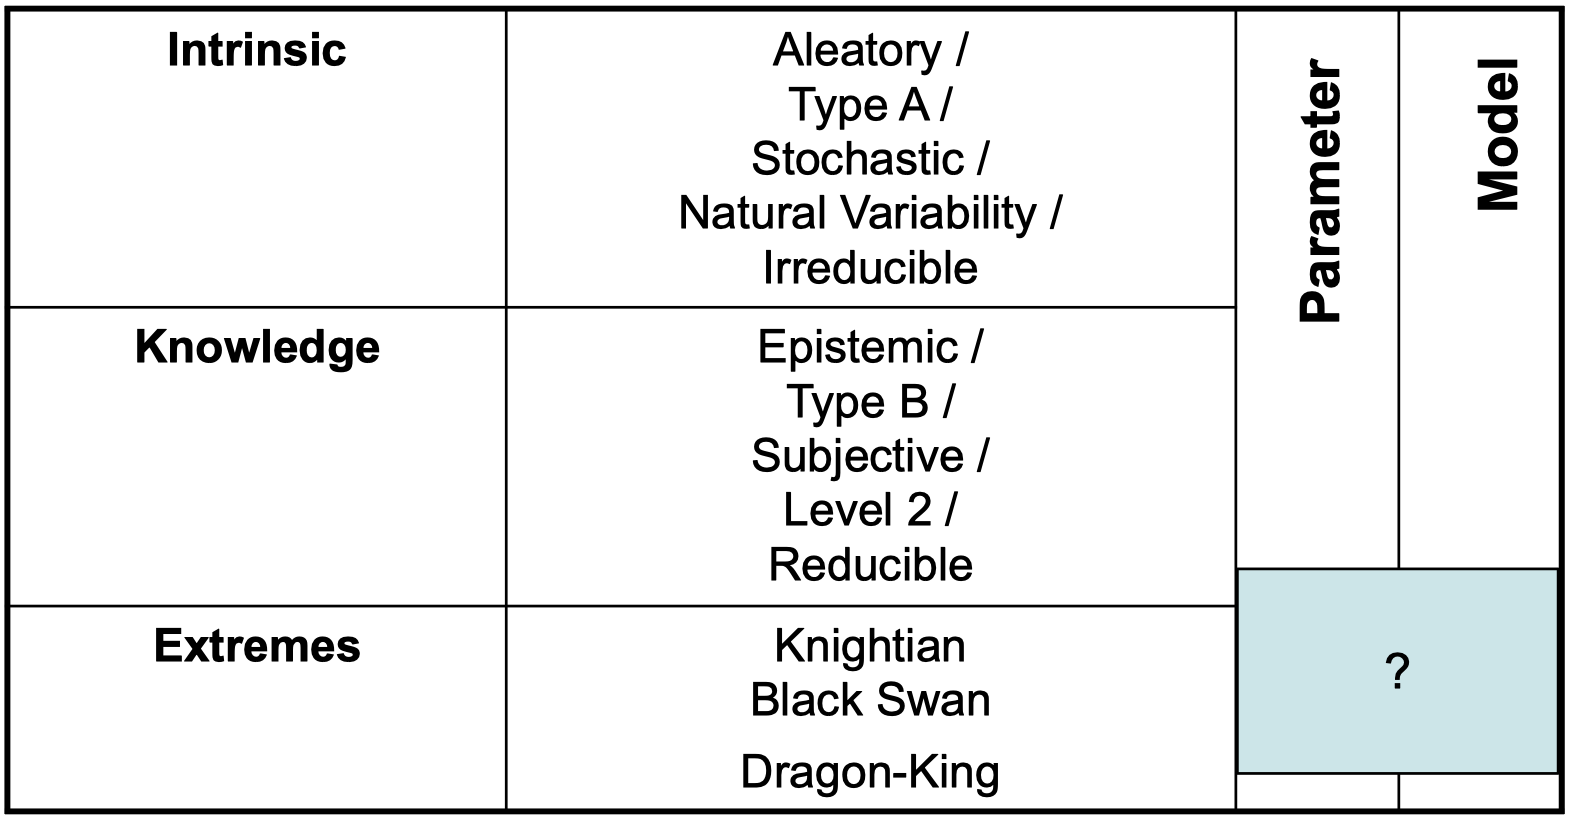
\includegraphics[width=10cm]{../images/EnpRisk_Fig1-1}
    \centering
\end{figure}

\end{document}